\documentclass{article}
\usepackage{pythonhighlight}
\usepackage{graphicx}
\usepackage{ctex}
\usepackage[left=3cm,top=3cm,right=3cm]{geometry}
\usepackage{hyperref}
% TITLE PAGE CONTENT %%%%%%%%%%%%%%%%%%%%%%%%
%%%%%%%%%%%%%%%%%%%%%%%%%%%%%%%%%%%%%%%%%%%%%
\newcommand{\labno}{05}
\newcommand{\labtitle}{EE208 Lucene}
\newcommand{\authorname}{周李韬}
\newcommand{\studentno}{518030910407}
\newcommand{\classno}{F1803016}
% END TITLE PAGE CONTENT %%%%%%%%%%%%%%%%%%%%


\begin{document}

\begin{center}
{\LARGE \textsc{Laboratory No. \labno:} \\ \vspace{4pt}}
{\Large \textsc{\labtitle} \\ \vspace{4pt}} 
\rule[13pt]{\textwidth}{1pt} \\ \vspace{15pt}
{\large By: \authorname \\ \vspace{10pt}
No. \studentno \\ \vspace{10pt}
SJTU \classno \\ \vspace{10pt}
\today \vspace{20pt}}
\end{center}



\section{实验准备}

\subsection{实验环境}
\begin{itemize}
\item\textbf{Environment} Ubuntu 16.04 (on Virtual Machine)
\item\textbf{Language} Python 2.7.16 with packages as follows
	\begin{itemize}
	\item urllib 1.24.2
	\item beautifulsoup4 4.8.0
	\item lucene 4.9.0
	\end{itemize}
\item\textbf{Tools} PyCharm 2019.2, Virtual Box
\end{itemize}

\subsection{实验目的}
本实验分为两部分,在第一部分,我们需要在原有搜索引擎的基础上加以改进,实现一个能够支持“site:”域名条件检索的搜索引擎。在第二部分,我们需要实现一个基于图片周围文本进行图片检索的搜索引擎。

\subsection{实验原理}
\label{sec:principle}

在第一部分的实验中,对域名检索而言,我们在Lab5中搭建的搜索引擎是不够的。这是因为该搜索引擎的索引中,并不存在我们需要检索的对象site,因此,我们需要更新原有的索引。在这里我们利用Lucene中的Term包匹配原来索引库中的文档,随后采用indexWriter中的deleteDocument()函数进行删除。再重新添加包含site域的索引文档。对检索程序部分,我们需要对输入的检索命令进行处理,提取其中分别对应site和content域的内容,并进行词法、语法分析,进而构造符合用户输入需求的query对象进行查询,才能实现满足实验目标的搜索引擎。

在第二部分的实验中,我们爬取了“豆瓣电影”(域名:movie.douban.com)站点下一定数量的电影、人物主页,针对页面的特征提取了这类网页上的主要电影、人物图片,将图片地址、网页URL、周边文字信息等信息有序地输出保存。随后,我们采用与此前实验类似的方法进行索引、搜索程序的构造,达到图片检索的目的。实验的具体实现细节将在下文展开。


\section{实验步骤}

\subsection{支持域名的搜索引擎}

\subsubsection{Solution}

解析包含“site:”条件的命令函数parsecommand()已在示例代码中给出并被本实验使用,对其他信息的处理、索引、搜索等过程已经在Lab4中实现,在本文中不再详述。

\paragraph{索引配置}
注意到网页的域名site内容是一个以“.”为间隔标记的若干英文字符串,因此中文分词器对site信息不会产生空格的分词效果,也就不会在analyzer阶段被WhiteSpaceAnalyzer识别。因此在本实验中,我们改用SimpleAnalyzer作为分词器,该分词器能够识别非字符的符号作为分词的依据,在这里既可以对中文空格进行分词,也可以对英文域名间的句点进行分词,满足本实验的要求。对于site的fieldType选择,由于它是用户的检索对象之一,因此也需要被索引、分词。此外,由于对域名的检索通常要求连续字段的匹配,因此在索引中记录词频和位置也是十分重要的,为了方便实验的检验,我们也将域名存储了下来,实际应用中是可以去除的。本实验中的fieldType配置如下表所示。
\begin{table}[h]
\begin{center}
\begin{tabular}{cccccc}
\hline
\textbf{Field Type} & \textbf{Field Name} & \textbf{Indexed} & \textbf{Stored} & \textbf{Tokenized} & \textbf{\begin{tabular}[c]{@{}c@{}}Record Freq\\ \& Position\end{tabular}} \\ \hline
\textbf{t1}         & path, url, name     & N                & Y               & N                  & N                                \\
\textbf{t2}         & contents            & Y                & N               & Y                  & Y                                \\
\textbf{t3}         & titles              & Y                & Y               & Y                  & Y                                \\
\textbf{t4}         & site                & Y                & Y               & Y                  & Y                                \\ 
 \hline
\end{tabular}
\end{center}
\end{table}

\paragraph{更新索引}
与Lab4中创建索引一样,我们通过遍历爬虫的结果目录index.txt对索引进行更新操作。更新索引的大部分代码与创建索引类似。不同之处首先在于我们要在创建新的索引前删除原有文档中的索引,我们利用Term工具匹配当前文件名对应的索引条目并删除。随后,我们为site域添加当前网页的域名,域名信息可以通过对当前URL调用urlparse库得到。更新索引的主要代码如下所示。

\begin{python}
def get_site(url):                                        # 从URL中提取域名
    return urlparse(url).netloc

def indexDocs(self, root, writer):
    while True:
        t = indextxt.readline()
        if (len(t) == 0):
            return
        ...
        URL = t[0]
        try:
            writer.deleteDocuments(Term("name", filename))# 匹配并删除当前文档的原索引
            ...
            doc.add(Field("site", get_site(URL), t4))     # 在索引文档中添加site域信息
            ...
        except Exception, e:
            print "Failed in indexDocs:", e
\end{python}

\paragraph{搜索程序}
实验材料中已为我们提供了一个处理用户输入的函数parsecommand(),它能将用户输入的命令转换成一个以检索field为key,以用户输入的关键词为value的dict数据结构。在此基础上,我们首先要对用户查询中文contents的关键词做分词处理,留待检索时被SimpleAnalyzer分词解析。随后对command\_dict进行遍历,将满足用户需求的field和keyword依次添加到最终用于检索的querys中,我们的添加结合方式为MUST,也就是说要同时满足所有条件的文档才会被输出。接下来用类似Lab4的方法,在此前构造的索引中对该querys进行检索,即可达到实验的目的。

\begin{python}
command_dict = parseCommand(command)                # 调用parsecommand函数,获得command_dict
seg_list = jieba.cut(command_dict['contents'])
command_dict['contents'] = (" ".join(seg_list))
querys = BooleanQuery()
for k,v in command_dict.iteritems():
    query = QueryParser(Version.LUCENE_CURRENT, k,
                        analyzer).parse(v)
    querys.add(query, BooleanClause.Occur.MUST)
\end{python}

\subsubsection{Results}

构造索引过程截图如图\ref{fig:siteindex}所示,搜索结果示例如\ref{fig:sitetest}所示,当限定域名为sh.sina.com.cn时,排在前列的搜索结果都是新浪上海域名下的网页。

\begin{figure}[htbp]
\centering
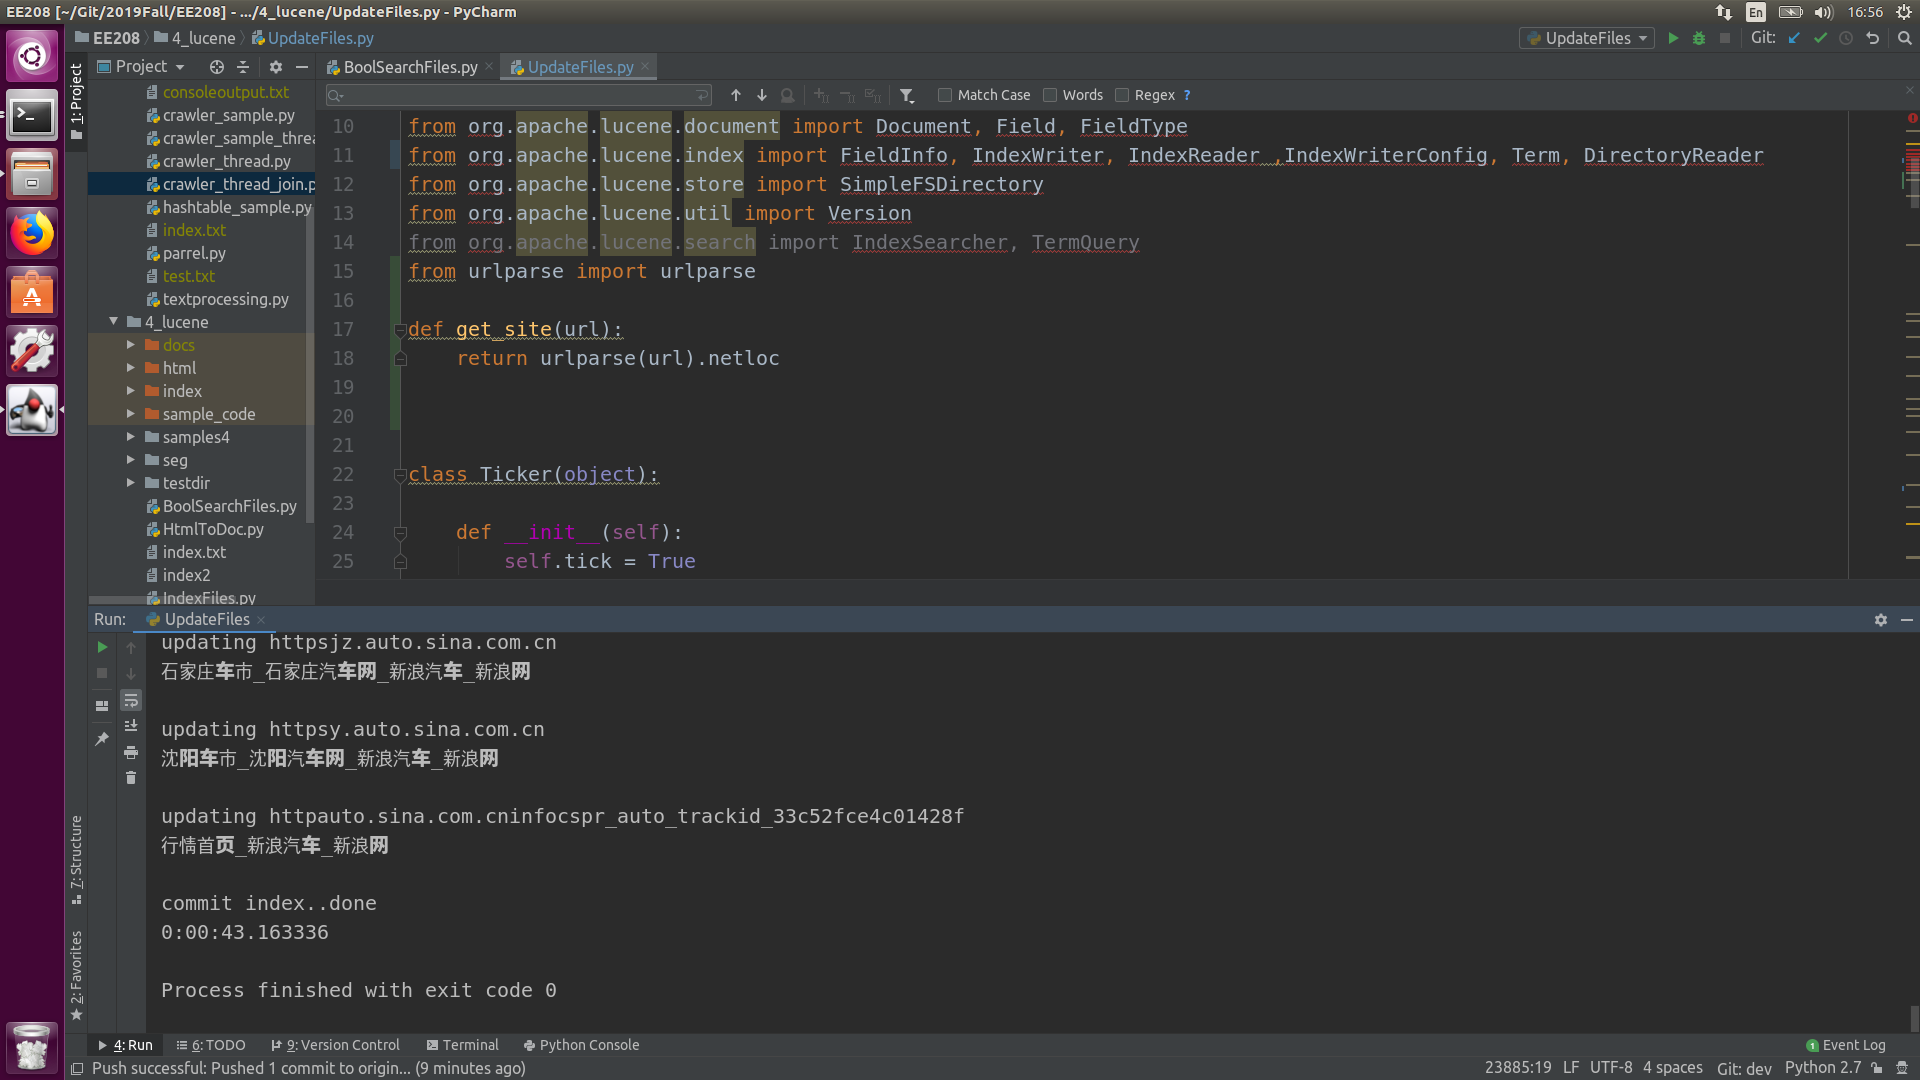
\includegraphics[width=14.5cm]{img/siteupdate.png}
\caption{构造索引过程}
\label{fig:siteindex}
\end{figure}


\begin{figure}[htbp]
\centering
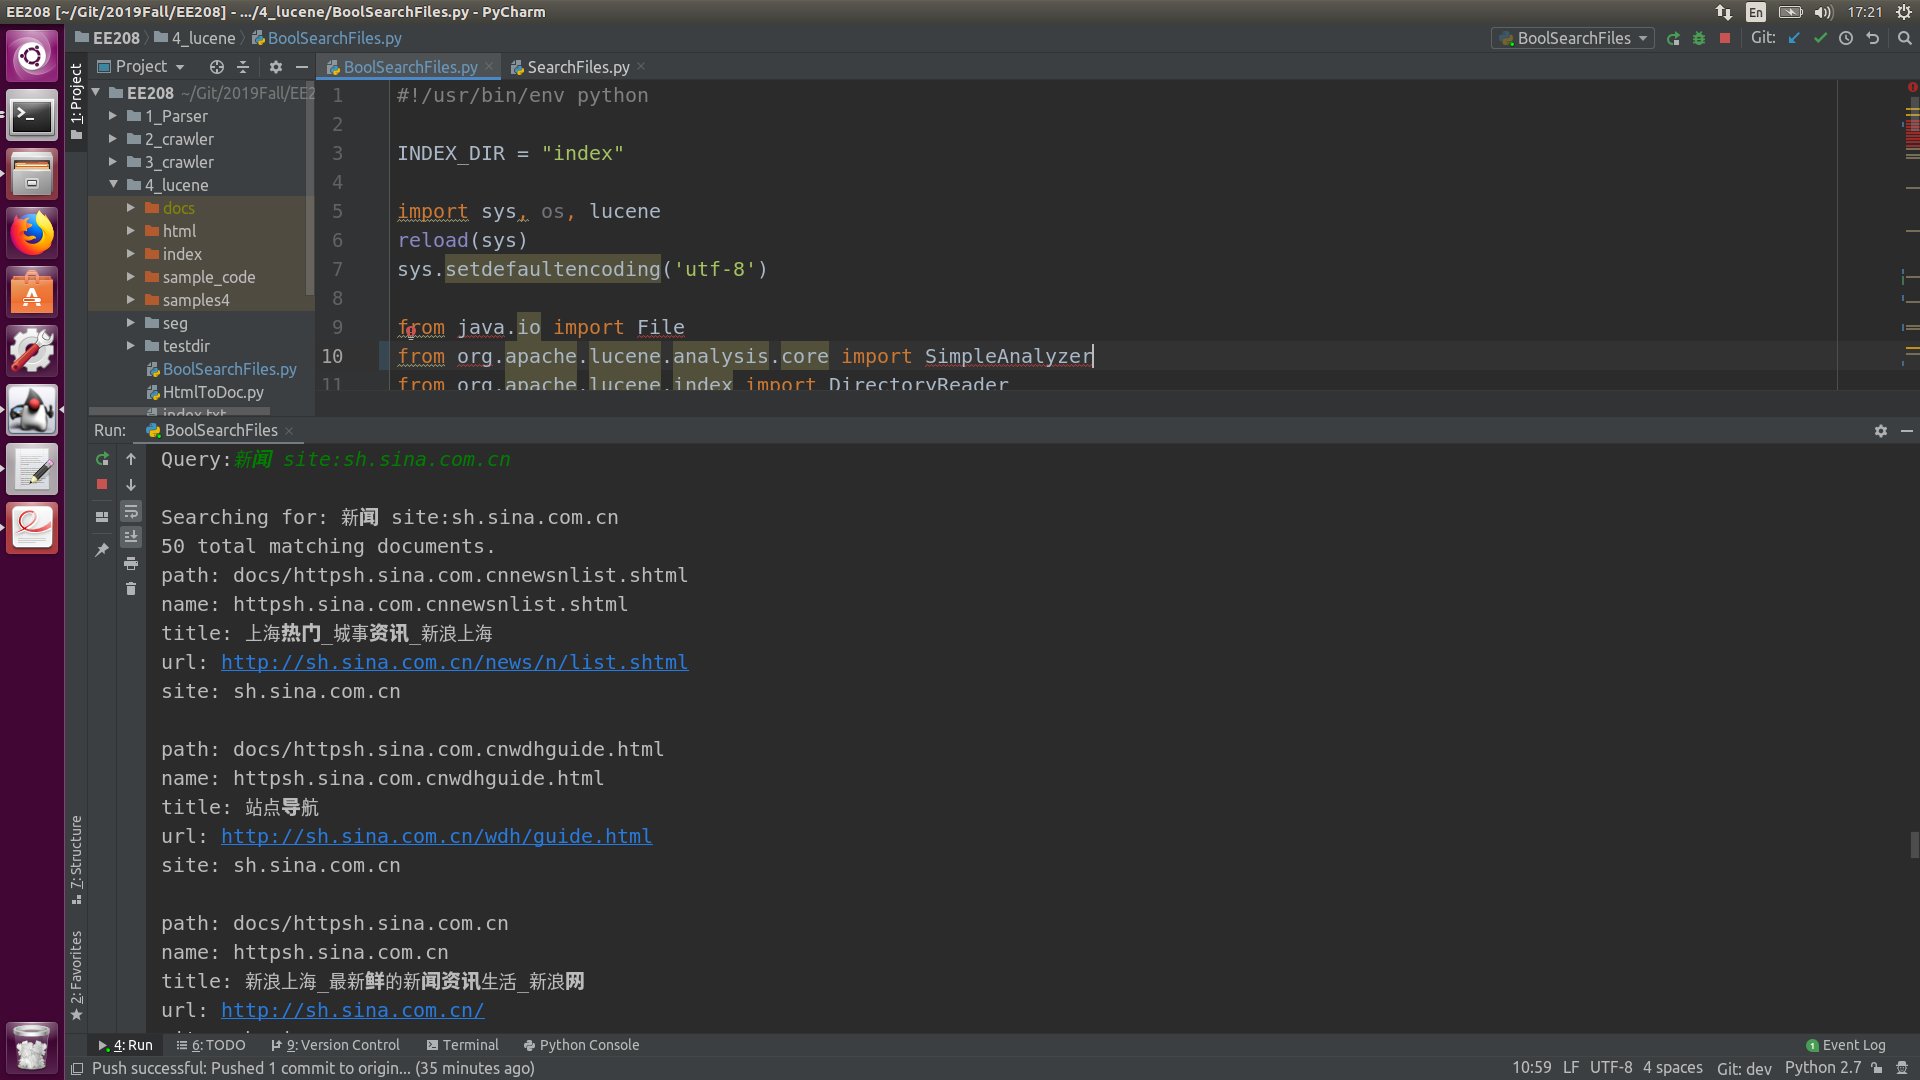
\includegraphics[width=14.5cm]{img/sitesearch2.png}
\caption{搜索结果示例}
\label{fig:sitetest}
\end{figure}




\subsection{图片搜索引擎}

\subsubsection{Solution}

\paragraph{爬取豆瓣电影网页}

\begin{python}
def URL_set_uniform(URLset,page):
    urlseg = urlparse.urlparse(page)
    uniURLs = set()
    for i in URLset:
        j = i['href'].split('#')[0]      # remove parameters
        ......                           # 将相对路径转化为绝对路径
        jseg = urlparse.urlparse(j)      # 获得当前页面的域名,仅当域名是豆瓣电影时加入队列
        if (jseg.netloc == 'movie.douban.com'):
            uniURLs.add(jseg.scheme+'://'+jseg.netloc+jseg.path)
    return uniURLs
\end{python}


\paragraph{提取图片信息}

\begin{python}
def extract_subject(soup, output):
    global COUNT
    title = soup.h1.get_text(strip=True).split('(')[0]          # 网页标题,去除(豆瓣)后缀
    titleseg = jieba.cut(title)
    title = ' '.join(titleseg)                                  # 对网页标题分词

    # 电影主题图
    output.write(soup.find(id = "mainpic").img['src']+'\n')     # 电影主题图地址打印在第一行
    output.write(title+' ')
    infoseg = jieba.cut(soup.find(id="info").get_text(strip=True))
    infos = " ".join(infoseg)              # title+infos作为电影相关信息的分词结果打印在第二行
    output.write(infos+'\n')
    COUNT += 1
    
    # 电影主要卡司
    for celebrity in soup.select(".celebrity"):
        imgsrc = celebrity.select('.avatar')[0]['style'].split('(')[1].split(')')[0]
        output.write(imgsrc+'\n')                               # 电影卡司人物图打印在第一行
        output.write(title+' ')
        textseg = jieba.cut(' '.join(celebrity.select(".info")[0].get_text().split('\n')))
        output.write(" ".join(textseg))                         # 电影卡司信息打印在第二行
        output.write('\n')
        COUNT += 1
        
    # 电影相关图
    related_session = soup.find(id = "related-pic")
    for pic in related_session.find_all('img'):
        imgsrc = pic['src']
        ...    # 在output中第一行写入imgsrc,第二行写入和标题图一样的title,infos等信息
        COUNT += 1

    output.write('EOF')
\end{python}


\paragraph{建立图片文档}
\begin{python}
# 一个用于获取豆瓣电影域名下页面类型(即path的第一级目录)的函数
def getPageType(URL):
    urlseg = urlparse.urlparse(URL)
    if len(urlseg.path)>0:
        return urlseg.path.split('/')[1]
    else:
        return ''
\end{python}

\begin{python}
def PagesToDocs(root,index,storeDir):
    while (True):
        从index的一行中获取URL,filename和pagetype,如果一行为空则break
        try:
            path = os.path.join(root, filename)
            content = open(path)
            soup = BeautifulSoup(content, features='lxml')
            content.close()
            if pagetype in ["subject","celebrity"]:
                output = open(os.path.join(storeDir, filename), 'w')
                从content中提取标题title
                在output中写入title,URL
                调用globals()['extract_%s' % pagetype](soup, output)
                将当前文件名写入docindex文件中
        except Exception, e:
            print "Failed in indexDocs:", e

if __name__ == "__main__":
    COUNT = 0                                # COUNT是一个全局计数器,统计被存储的图片数
    PagesToDocs("html","index.txt","docs")
    print "total images collected", COUNT
\end{python}




\paragraph{图片索引与搜索}

\begin{table}[h]
\begin{center}
\begin{tabular}{cccccc}
\hline
\textbf{Field Type} & \textbf{Field Name} & \textbf{Indexed} & \textbf{Stored} & \textbf{Tokenized} & \textbf{\begin{tabular}[c]{@{}c@{}}Record Freq\\ \& Position\end{tabular}} \\ \hline
\textbf{t1}         & imgurl, url, name   & N                & Y               & N                  & N                                                                          \\
\textbf{t2}         & contents            & Y                & N               & Y                  & Y                                                                          \\
\textbf{t3}         & titles              & Y                & Y               & Y                  & Y                                                                          \\ \hline
\end{tabular}
\end{center}
\end{table}


\subsubsection{Results}

\begin{figure}[htbp]
\centering
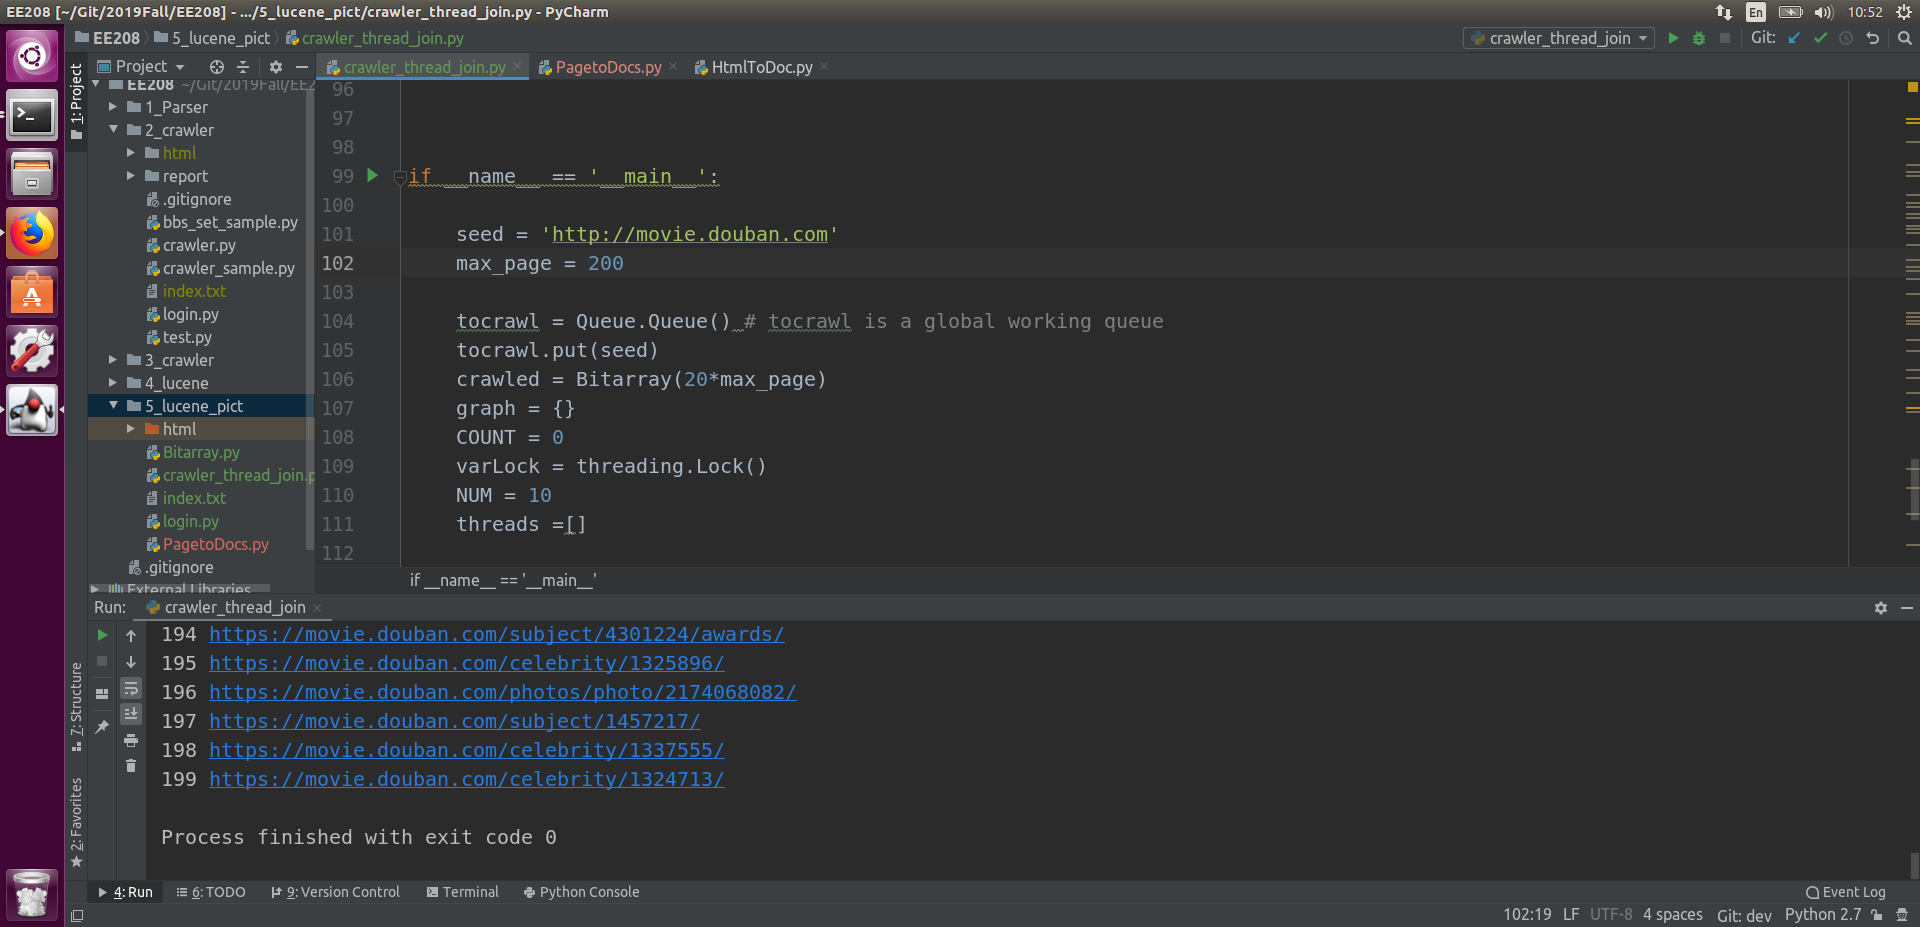
\includegraphics[width=14.5cm]{img/crawl_images.png}
\caption{爬取豆瓣电影网页过程截图}
\label{fig:crawl_images}
\end{figure}

\begin{figure}[htbp]
\centering
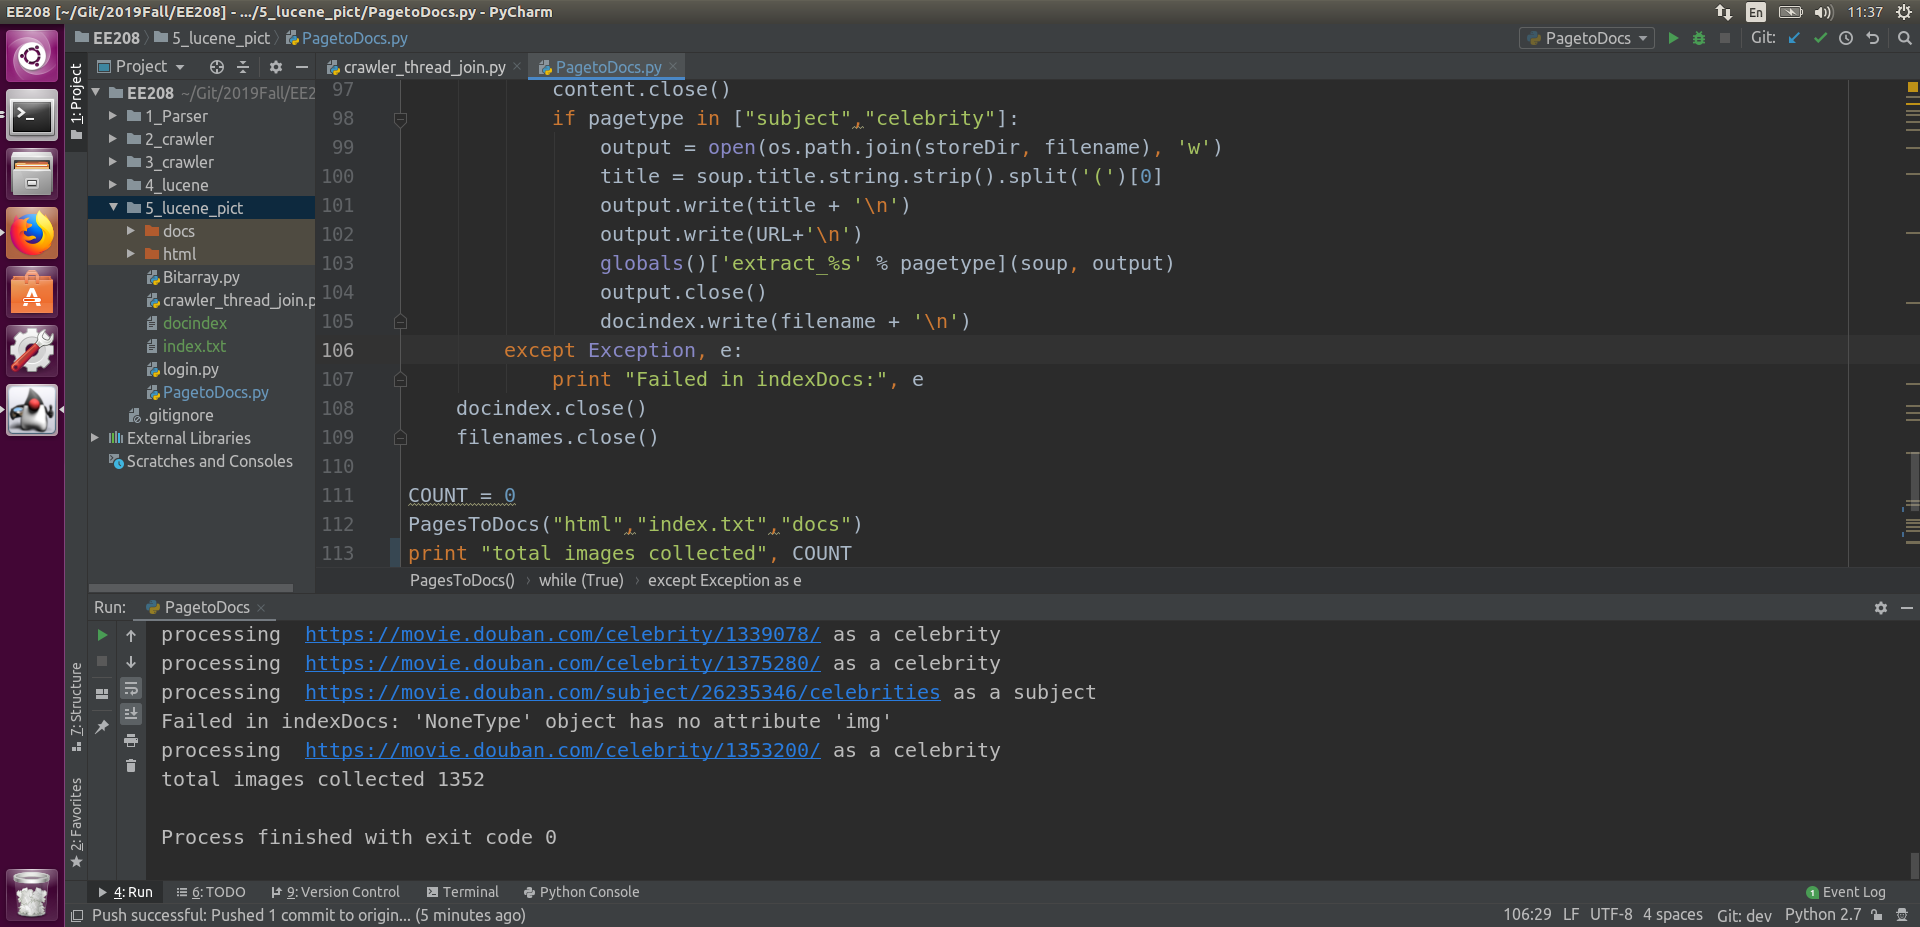
\includegraphics[width=14.5cm]{img/getpict.png}
\caption{建立图片文档过程截图}
\label{fig:pagetodocs}
\end{figure}

\begin{figure}[htbp]
\centering
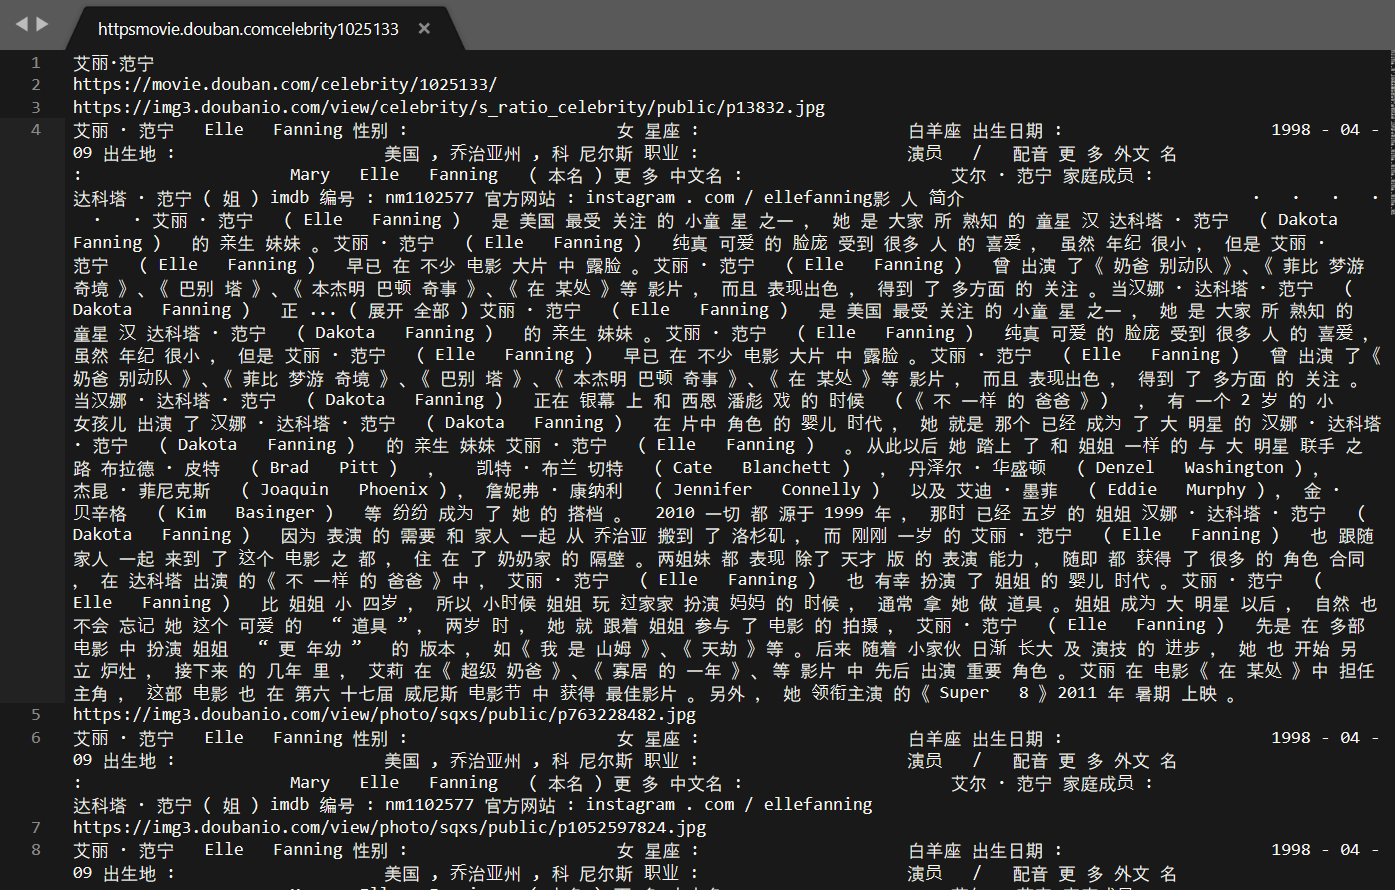
\includegraphics[width=14.5cm]{img/pictdocs.png}
\caption{图片文档结果示例}
\label{fig:docexample}
\end{figure}

\begin{figure}[htbp]
\centering
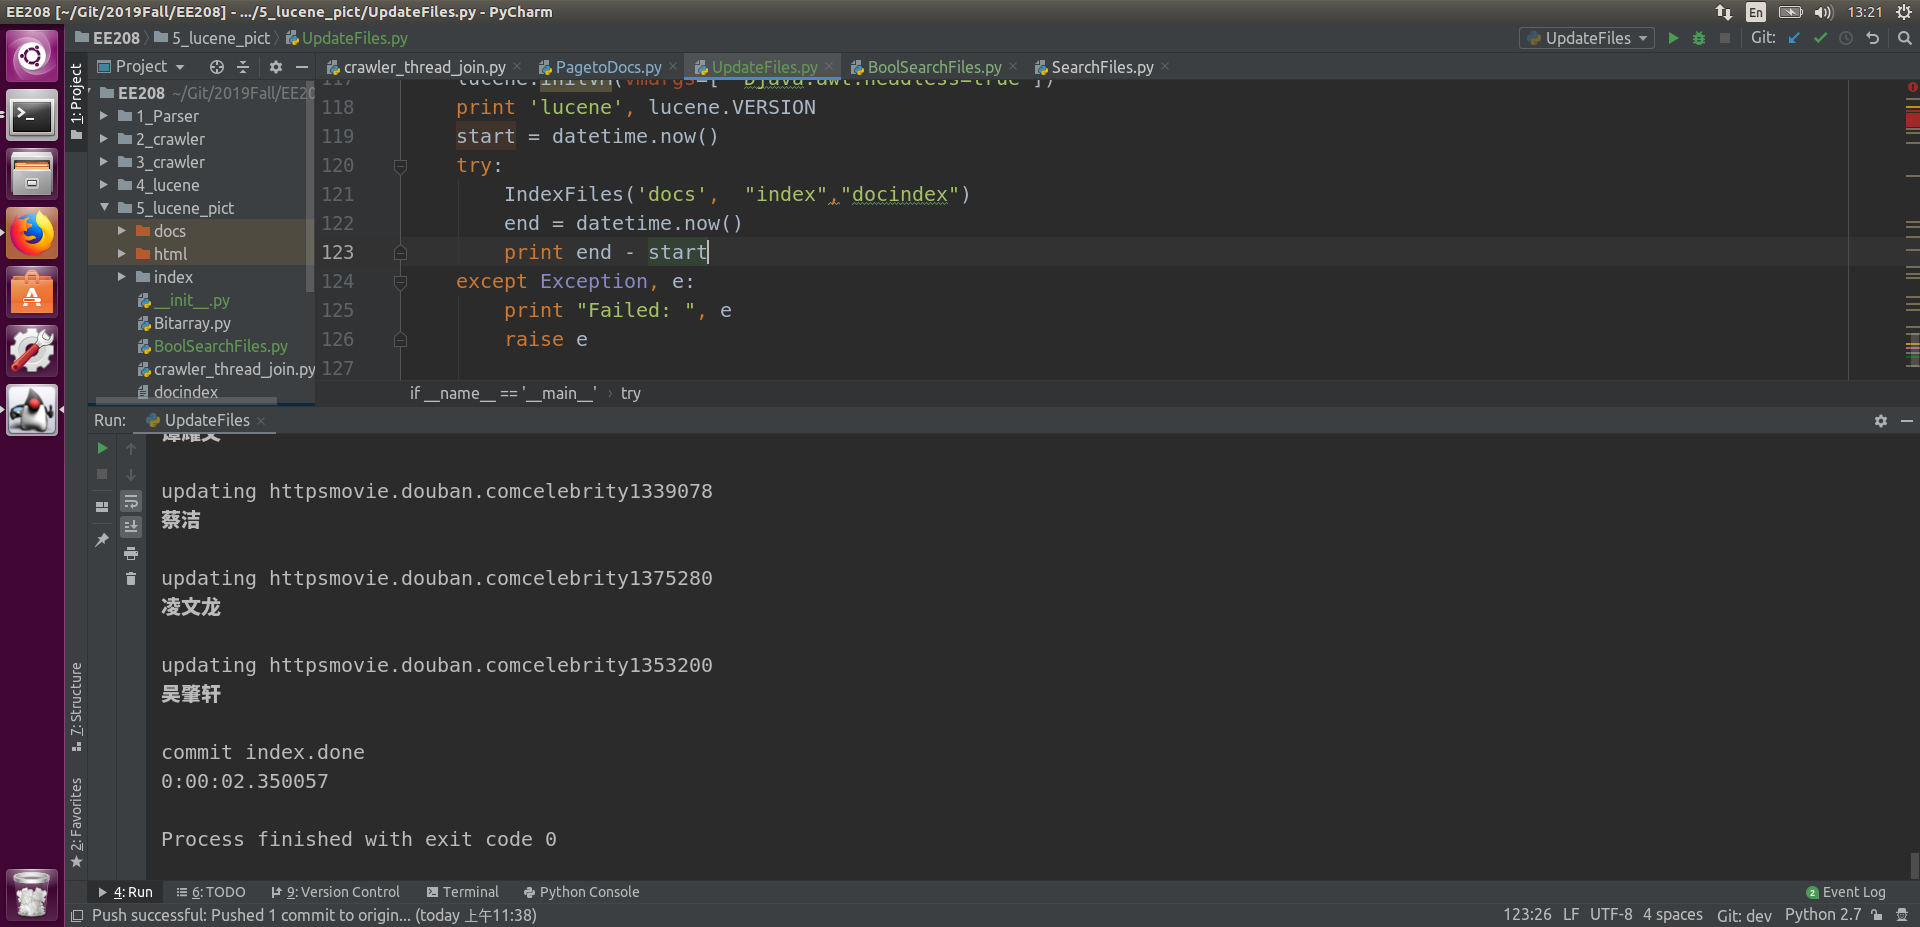
\includegraphics[width=14.5cm]{img/indexing.png}
\caption{为图片文档建立索引过程截图}
\label{fig:indexpict}
\end{figure}

\begin{figure}[htbp]
\centering
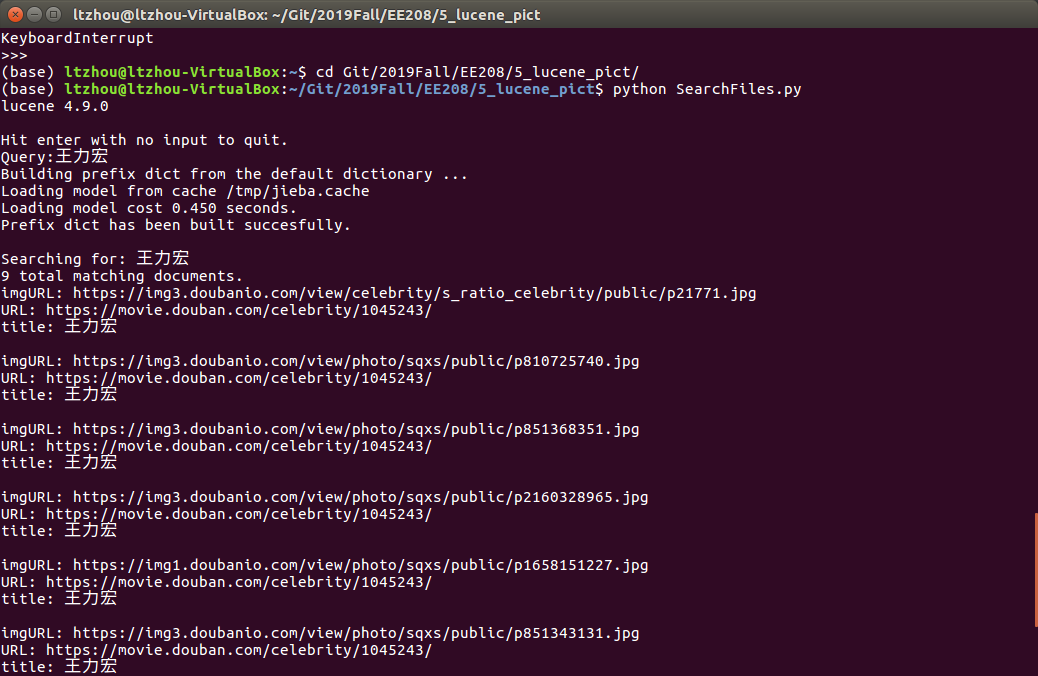
\includegraphics[width=8.5cm]{img/search.png}
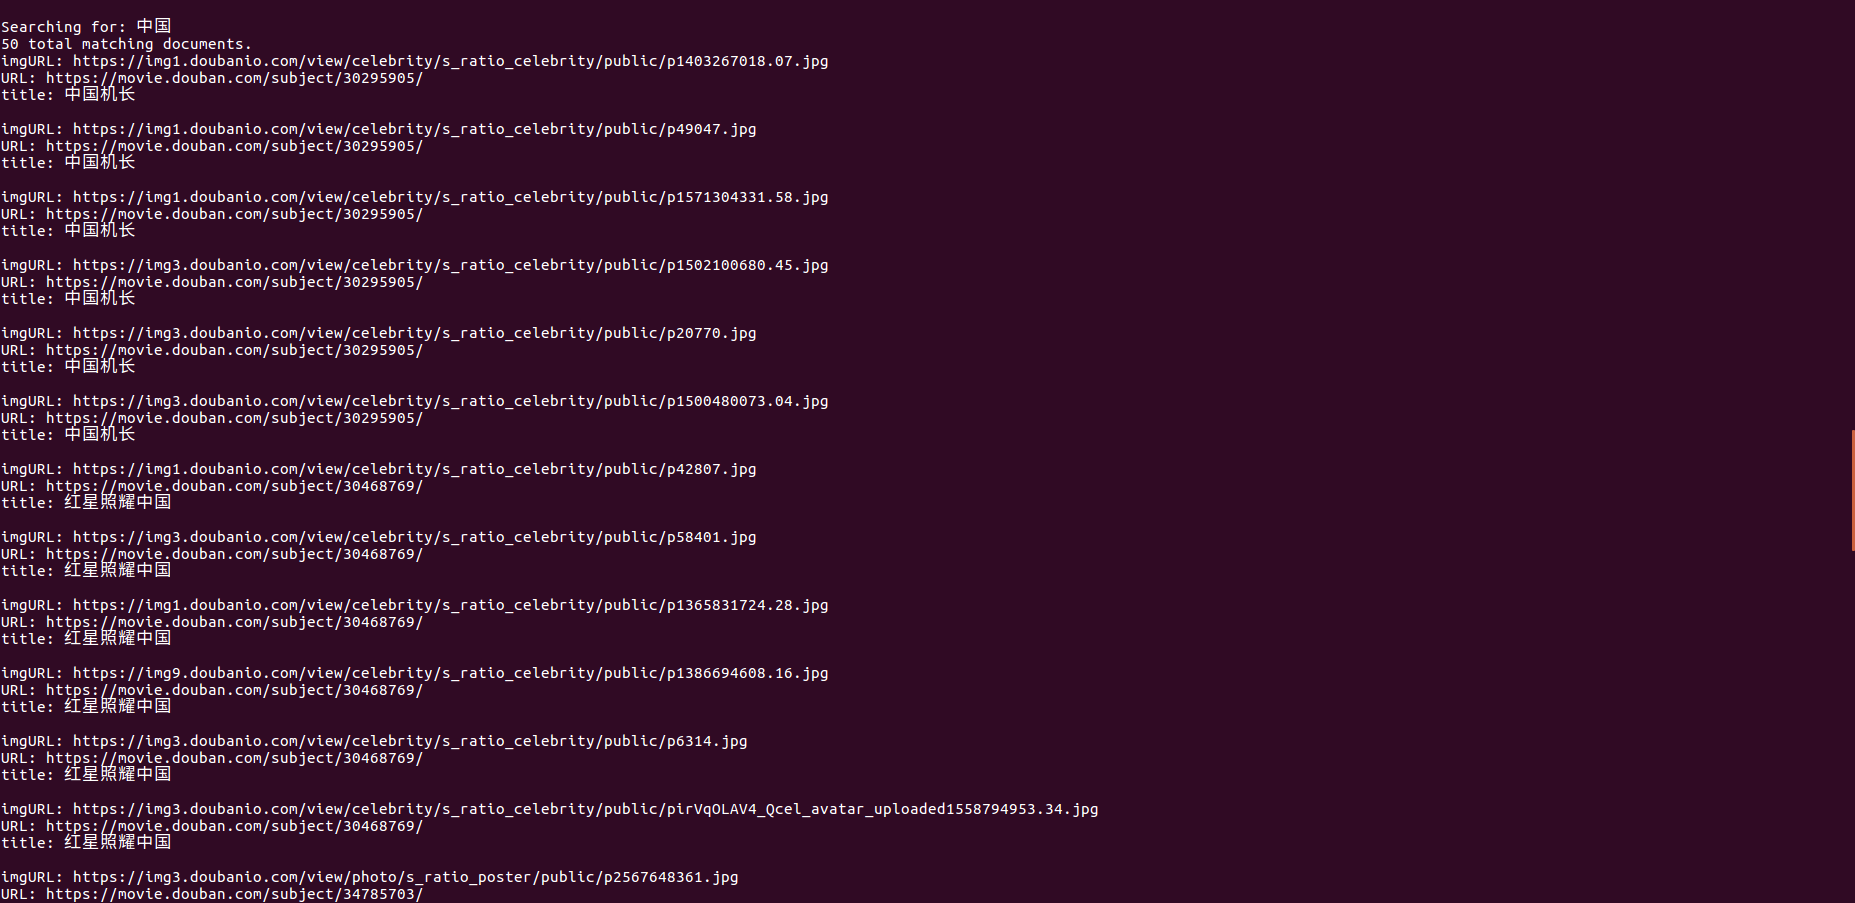
\includegraphics[width=8.5cm]{img/search2.png}
\caption{图片搜索示例}
\label{fig:search1pict}
\end{figure}

\begin{figure}[htbp]
\centering
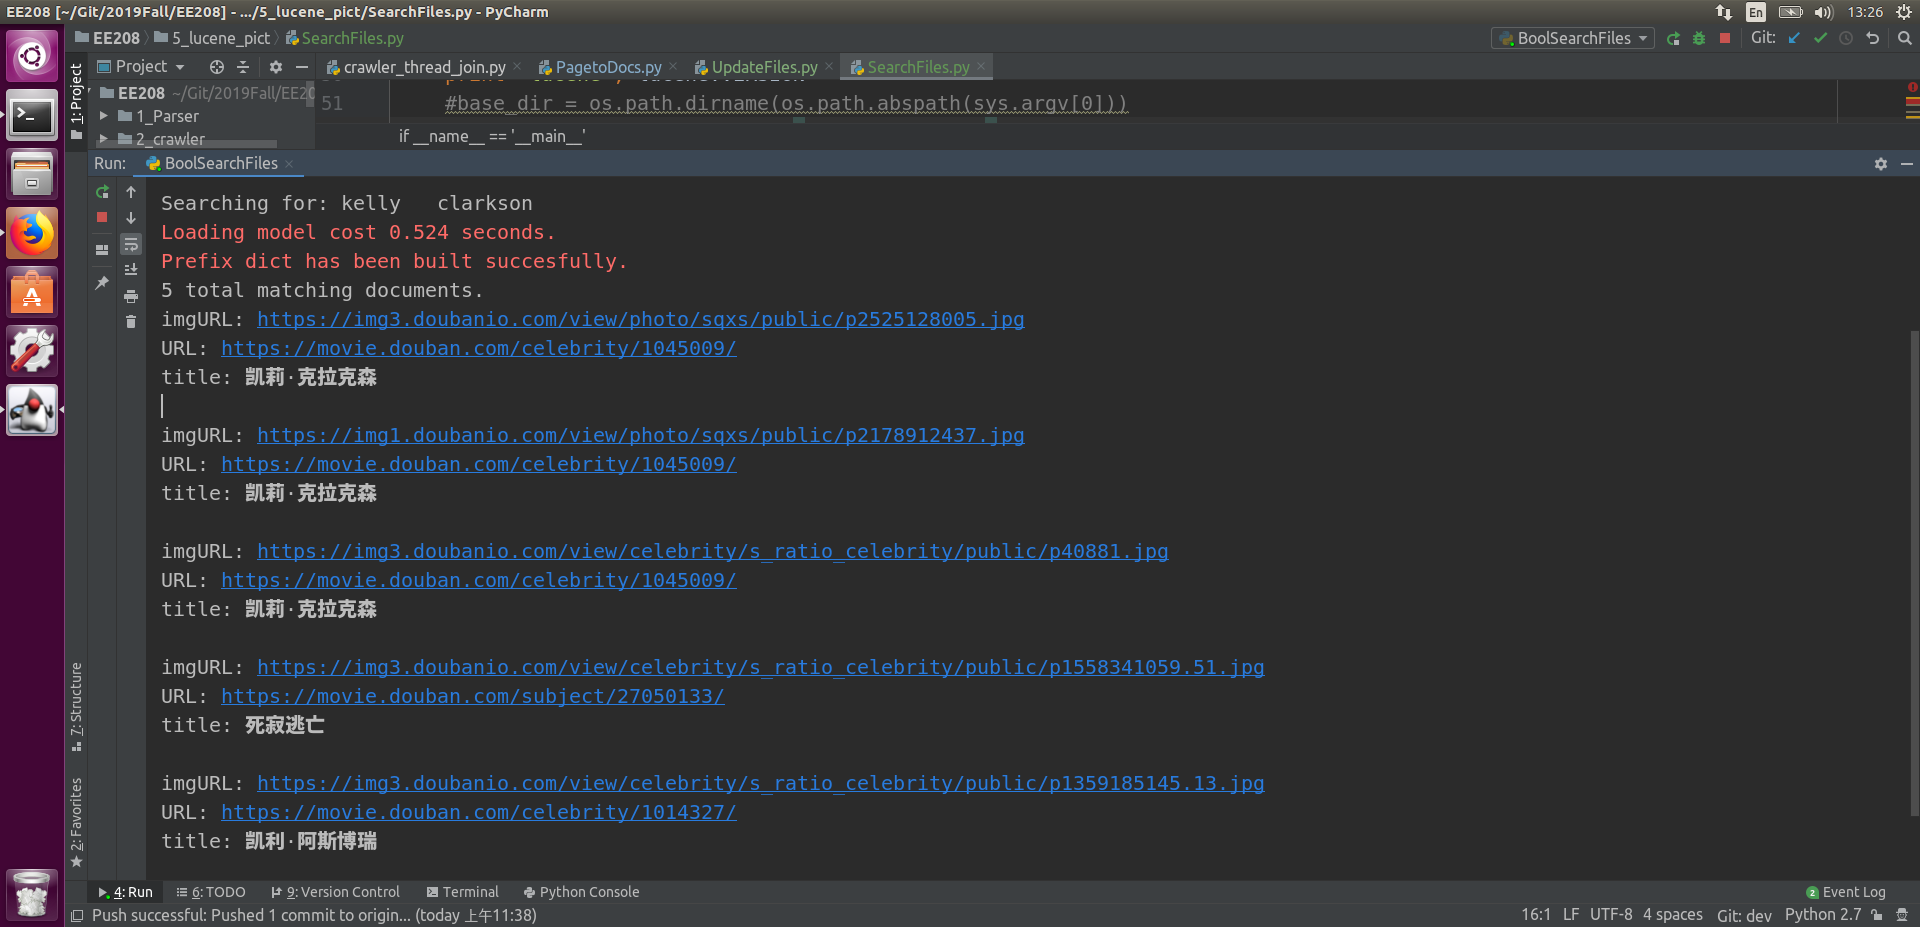
\includegraphics[width=14.5cm]{img/search3.png}
\caption{图片搜索示例}
\label{fig:search2pict}
\end{figure}

\section{实验总结}
\paragraph{概述}
通过本次实验的学习,我将课堂上学习到的建立索引表、词法分析、文档打分等概念付诸实践,学会了如何利用lucene搭建一个简单的搜索引擎。

\paragraph{感想}
为了提高搜索引擎的检索效果,构建索引的过程十分重要,我们的索引应该能够完备、有效地描述一个网页中主要的文字内容。在最初,我使用了一个简单的get\_text函数提取网页上的文本,这样做所带来的问题是我们所提取出的文字中,大量javascript、CSS代码被识别成文本保留了下来,对这些代码做索引是没有意义的,这将降低搜索引擎的表现。在通过网络获得帮助,对提取文本的函数经过改进后,我们的中文搜索引擎能够达到良好的检索效果。这带给我的启示是在对网页建立索引时,我们需要灵活根据需要提取有用的信息,避免冗余信息影响索引的构建和检索的效果。

\paragraph{创新}
在本实验中,我新建了一个将中文网页提取文本、进行分词的函数(HtmltoDoc.py)。该函数能够将一个目录下的HTML文件进行解析,提取出其中的文本,并利用结巴分词器进行分词,将分词结果输出在另一个目录下的同名文件中。该函数能够独立地被调用,用于网页信息的预处理、检索索引的建立等场合中。


\paragraph{问题}
本实验在处理site检索过程中,遇到的一个问题是域名无法做到部分匹配。如输入site:sina. com.cn时,只会输出域名是sina.com.cn的网址,其他类似www.sina.com.cn的网页不会被输出,如图\ref{fig:sitetest2}所示。分析原因,我们原本采用的分词器是WhiteSpaceAnalyzer,这一分词器能对我们经过空格分隔的中文分词结果有效,但并不会对网站域名做任何分词的操作,因此我们改用SimpleAnalyzer解决了这一问题。这一问题的出现和解决提示我们在构造索引的过程中,选择合适的分词方式十分重要,这极大关系到搜索引擎的效率、表现乃至正确率。

\begin{figure}[htbp]
\centering
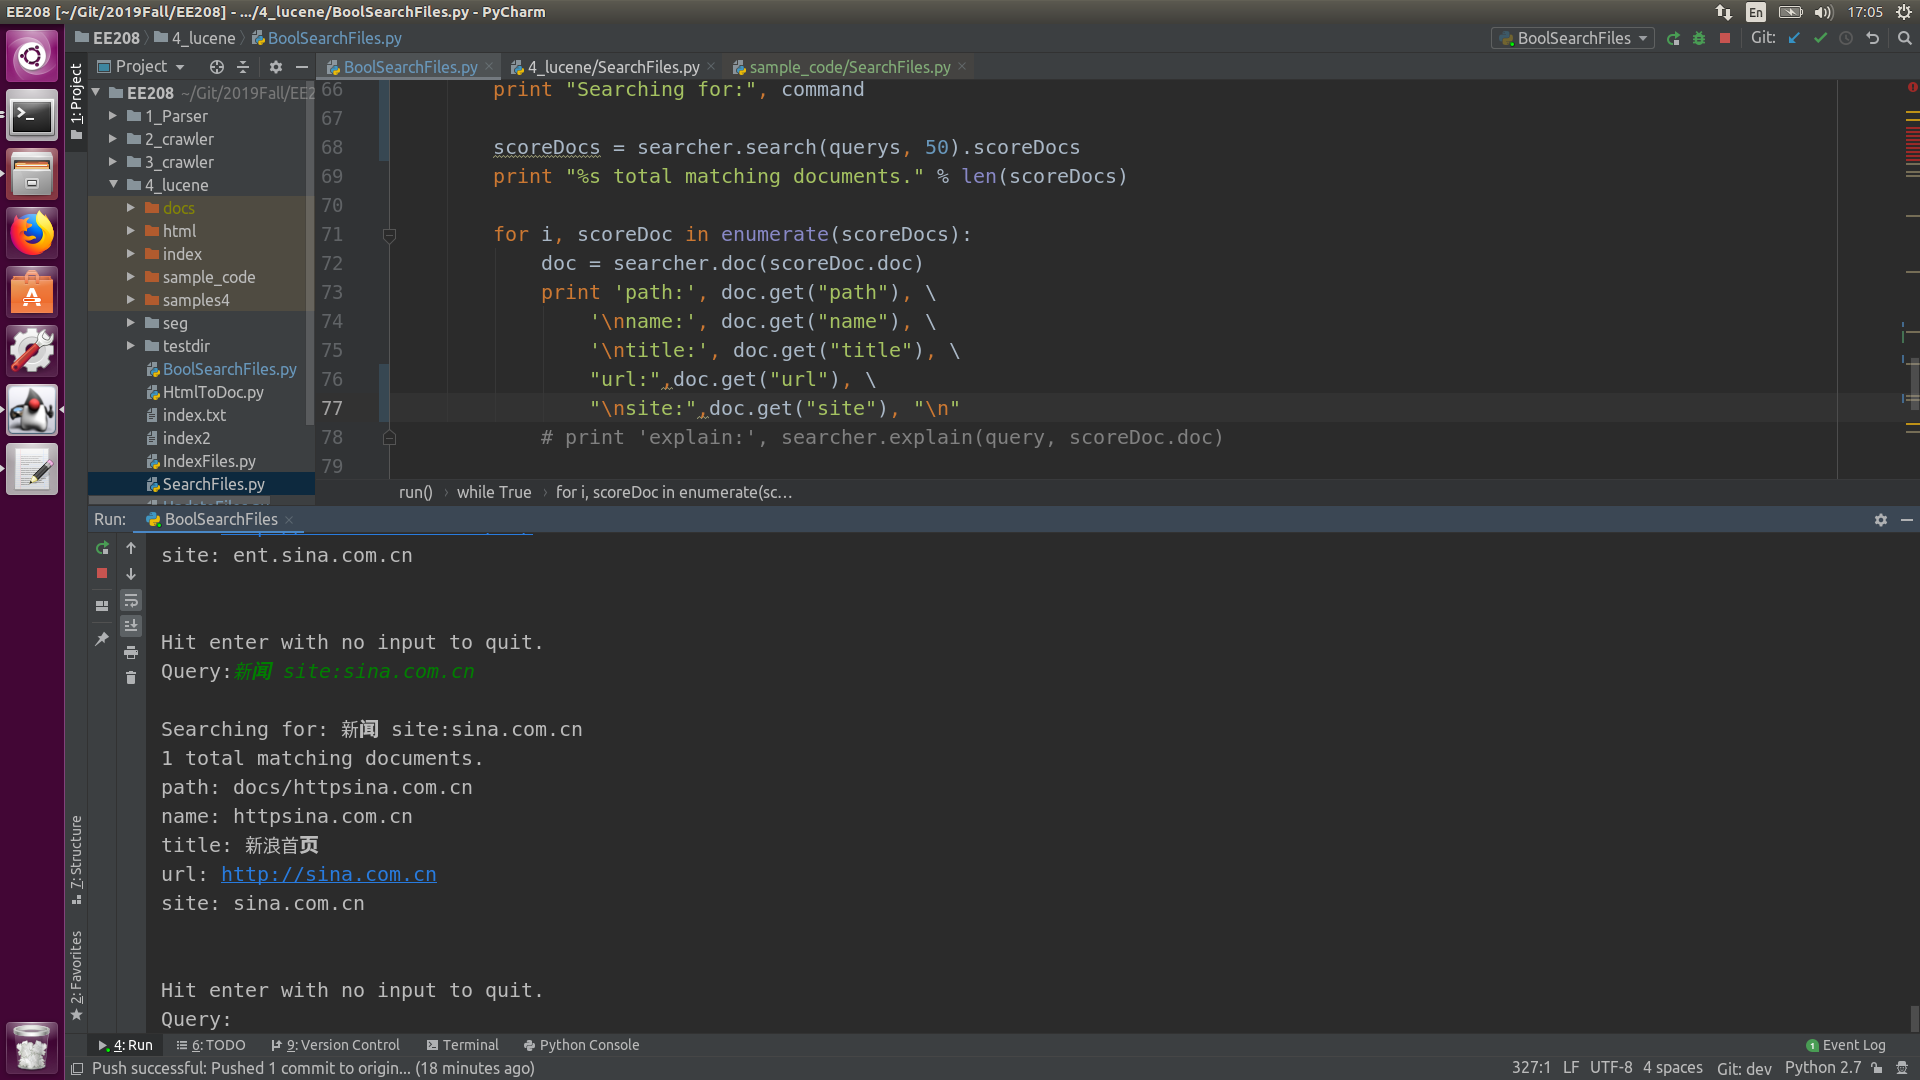
\includegraphics[width=14.5cm]{img/sitesearch.png}
\caption{使用WhiteSpaceAnalyzer的检索结果}
\label{fig:sitetest2}
\end{figure}



\end{document}

